\documentclass{article}
\usepackage[utf8]{inputenc}
\usepackage{natbib}
\usepackage{graphicx, caption, amsmath, amssymb}
\newcommand*{\myfont}{\fontfamily{lmtt}\selectfont}
\title{PhyloDivNet}
\author{Trinh & Willis}
\date{June 2019}


\begin{document}

\maketitle
\section{Introduction}
UniFrac. It's the unique fraction of branch lengths. So unique. 

If the goal is to generalize our results, then we need to include biological replicates in our sequencing. 

SO traditionally what's being done is that we get some data and then we calculate these relative abundances. Those relative abundances are from one sample time point with uncertainty around the biological variation. So we have that layer of uncertainty with our sampling methods and we want to try to get at a better estimate of the true relative abundance. So classically we take that data then use it to get at some measure of composition differences between individual samples. From there we take those distances from pairwise samples and we do hypothesis testing to see if there are differences in the distances between groups. 

So what do we want to do instead. What we want to do instead is take our data and we do a log ratio transformation that we can then use to model the data under a multivariate normal distribution. We fit a model with appropriate beta parameters based on our covariates of interest and then we log transform our mean values for each taxa with each grouping. From there what we get are mean relative abundances by grouping of interest. So we apply those mean relative abundances for each group to create some kind of group metric of weighted UniFrac. With that group metric of weighted UniFrac and variane estimates/confidence intervals around each of the mean weighted UniFrac distances between each pairwise group. 

ASK: How would hypothesis testing get implemented in this case? So what we would get is a UniFrac distance between groups of samples with some variance estimation around each mean UniFrac distance between groups. 
\section{Methods: Beta Diversity}


\subsection{UniFrac}

Weighted UniFrac is a quantitative phylogenetic diversity index and as such utilizes abundance information and a phylogenetic tree in its calculation. We start with samples from $i = 1,..., n$ ecosystems that have a known vector of covariates $X_i \in R^p$. $Q$ represents the number of species present in one or more ecosystems and we use $q = 1,...,Q$ to index the $Q$ taxa across all ecosystems. $Z_{iq} [0,1]$ refers to the latent relative abundance of taxon $q$ in ecosystem $i$ with the relative abundances of all taxon $q$ in ecosystem $i$ summing to 1. For each ecosystem $i$ there are $M_i$ total sequence counts observed that have been classified into $q$ taxa. $W_{iq}$ will represent the number of observed counts of taxon $q$ in ecosystem $i$. 

For the phylogenetic tree, let $m = 1,..., M$ index the branches of the phylogenetic tree where $M$ represents the total number of branches of the phylogenetic tree. $b_m$ denotes the branch length of the $nth$ branch. $d$ is the distance from each taxon $q$ to the root. And let $S_m$ represent the set of taxa that are descendents from branch $m$. 

The weighted UniFrac (Lozupone et. al 2007) diversity metric is defined as
\begin{equation}
    \hat{\beta}_{ij,WU,plug-in}=\sum_{i=1}^n b_n |\sum_{q \in S_{in}} \frac{W_{iq}}{M_i}-\sum_{q \in S_{jn}} \frac{W_{jq}}{M_j}| 
\end{equation}
Based on Eq. 1, the target estimand for weighted UniFrac is
\begin{equation}
    \beta_{ij,WU}=\sum_{i=1}^n b_n |\sum_{q \in S_{in}} Z_{iq} -\sum_{q \in S_{jn}} Z_{jq}| 
\end{equation}
To our knowledge, there has been no discussion of the target estimand for weighted UniFrac in the literature to date. There also exists a normalized weighted UniFrac metric where $\beta_{ij,WU} \in [0,1]$.  The normalized UniFrac plug-in estimate divides the weighted UniFrac by the average distance of each taxon $q$ from the root. 
\begin{equation}\label{eq:plugin}
    \hat{\beta}_{ij,NWU,plug-in}=\frac{\sum_{i=1}^n b_n |\sum_{q \in S_{in}} \frac{W_{iq}}{M_i}-\sum_{q \in S_{jn}} \frac{W_{jq}}{M_j}|}{\sum_{q=1}^Q d_q (\frac{W_{iq}}{M_i}+\frac{W_{jq}}{M_j})} 
\end{equation}
The target estimand for normalized weighted UniFrac is therefore 
\begin{equation}
    \beta_{ij,NWU}=\frac{\sum_{i=1}^n b_n |\sum_{q \in S_{in}} Z_{iq}-\sum_{q \in S_{jn}} Z_{jq}|}{\sum_{q=1}^Q d_q (Z_{iq}+Z_{jq})} 
\end{equation}

Compositional data can be modeled using a multinomial distribution where the covariances between components are negative constrained. If the sum of all components is equal to some known fixed $n$, an increase in one component will result in a decrease in another component and therefore be negatively correlated. To address this negative constrained covariance issue we follow the {\myfont DivNet}(Willis and Martin[under review]) approach to estimating the latent composition matrix $Z \in R^{nxQ}$ and beta-diversity. {\myfont DivNet} uses Aitchison’s log-ratio methodology to estimate the latent composition matrix by first modeling $W_{iq}$ from a multinomial distribution, 
\begin{equation}
p(W|Z)\propto\prod_{i=1}^n \prod_{q=1}^Q Z_{iq}^{W_{iq}}
\end{equation}
and then performing the log-ratio transformation by fixing some baseline taxon D as a comparison group: 
\begin{equation}
    Y_{iq}=\phi{Z_{iq}}=\{log(\frac{Z_{iq}}{Z_{iD}})\}_{q=1,...,D-1,D+1,...Q}
\end{equation}
Note that the log-ratio transformation is invertible $Z_{iq}=\phi^{-1}{Y_{iq}}$. The log-ratios $Y_{i}$ are then modeled using a multivariate normal distribution. We link the mean of $Y_i$ to covariates using $\mu_{i}=X_{i}^T\beta$. Our expected value of $Y_i$ can therefore be expressed as 
\begin{equation}
    \hat{Y_i} = X_{i}^T \hat{\beta}
\end{equation}
where $\hat{\beta}$ is the maximum likelihood estimate of $\beta$. The expected value of our random variable $Y_i$ can then be used to derive the fitted values of the latent composition since $\hat{Z}_i=\phi^{-1}(Y_i)$. 

Using {\myfont DivNet}'s estimation approach of $\beta$-diversity we propose the following estimate of weighted UniFrac and normalized weighted UniFrac 
\begin{equation}
\hat{\beta}_{ij,WU,proposed}=\sum_{i=1}^n b_n |\sum_{q \in S_{in}} \hat{Z}_{iq} -\sum_{q \in S_{jn}} \hat{Z}_{jq}| 
\end{equation}
\begin{equation}
    \hat{\beta}_{ij,NWU,propose}=\frac{\sum_{i=1}^n b_n |\sum_{q \in S_{in}} \hat{Z}_{iq}-\sum_{q \in S_{jn}} \hat{Z}_{jq}|}{\sum_{q=1}^Q d_q (\hat{Z}_{iq}+\hat{Z}_{jq})} 
\end{equation}

Here we define an estimand for weighted UniFrac and a proposed method which we call {\myfont PhyloDivNet} for estimating the weighted UniFrac estimand. 

\textbf{FLAG:: Go back through this to see what needs to be built out and if this is coherent}

\subsection{Phylogenetic Tree Construction}
\textbf{Note: I thought it would be good to have some mention of the tree and how we're assuming the tree that we input into PhyloDivNet is the best we can get, but that choice of tree will influence UniFrac}

A phylogenetic tree is a data structure that highlights evolutionary relationships between organisms. These relationships may be based on differences or similarities of genetic or physical characteristics. Construction of a phylogenetic tree is no trivial feat and is commonly approached using either distanced based i.e. UPGMA, neighbor-joining or character based i.e. maximum likelihood, maximum parsimony algorithms (REF).  Tree estimation using a maximum likelihood approach finds the tree that best explains the data by selecting the tree with the highest likelihood as the best tree. This is, however, an NP complete problem with large alignments (REF FastTree 2). As such, different algorithms such as PhyML and RAxML will start with a reference tree and try to maximize the likelihood by rearranging branches and optimizing branch lengths... 
...We assume that the phylogenetic tree that we construct is correct. 

\textbf{Pauline TO-DO: Need to develop out this section more.}


\subsection{Variance Estimation}
Accurate estimation of the variance of UniFrac estimates has important implications towards valid hypothesis testing. Variance estimation of our UniFrac estimates is carried out using parametric and nonparametric bootstrap approaches and evaluated under simulation. 
Parametric bootstrapping to estimate the $Var(\widehat{UniFrac_{ij}})$ is conducted as follows: 
Let $\hat{\beta}$ and $\hat{\Sigma}$ be the estimates of $\beta$ and $\Sigma$ of our log-ratio model and $B$ represent the number of bootstrap iterations. We simulate $B$ number of datasets from the log-ratio model using our $\hat{\beta}$ and $\hat{\Sigma}$ estimates.  For each simulated dataset $b=1,...,B$ we use {\myfont DivNet} to estimate the $\hat{\beta}^{b}$ and $\hat{\Sigma}^{b}$. From there,  we estimate the weighted UniFrac ($\widehat{UniFrac}_{ij}^{b}$) for $b=1,...,B$. The $\widehat{Var}(\widehat{UniFrac_{ij}^{b}})$ is therefore the parametric bootstrap estimate of the $Var(\widehat{UniFrac_{ij}})$.

Nonparametric bootstrapping to estimate the $Var(\widehat{UniFrac_{ij}})$ begins with some dataset $(W,X)$. We define $n_{sub}$ as the number of samples we want to subsample from the dataset (W,X) and let $i = 1,...,I$ index the samples. We then use a uniform random selection of $n_{sub}$ elements from ${1,...,n_{sub}}$ that will correspond to the sample indices subsampled from some dataset $(W,X)$. The subsampled set of samples will be referred to as $P$. With each set $P$ we estimate $\hat{\beta}^{P}$ and $\hat{\Sigma}^{P}$ to obtain $\widehat{UniFrac_{ij}^{P}}$. We repeat this subsampling from (W,X) and estimation of $\widehat{UniFrac_{ij}^{P}}$ for $B$ iterations until we obtain a set of UniFrac estimates $\widehat{UniFrac_{ij}^{P_{b}}}$ for $b = 1,...,B$ bootstrap iterations. From there we obtain the nonparametric bootstrap estimate of $Var(\widehat{UniFrac_{ij}})$ by calculating $\widehat{Var}(\widehat{UniFrac_{ij}^{P_{b}}})$. 

\subsection{Simulation Study}
To examine the performance of {\myfont PhyloDivNet} we compare our proposed method against the  \textit{empirical plug-in} estimator (Vu et al. 2007) and the \textit{zero-replace} estimator (Mart\'in-Fern\'andez et al. 2003). The  \textit{empirical plug-in} estimator estimates the weighted UniFrac between ecosystems \textit{i} and \textit{j} by replacing $Z_{iq}$ and $Z_{jq}$ with the observed or empirical relative abundances $\frac{W_{iq}}{Mi}$ and $\frac{W_{jq}}{Mj}$. The \textit{empirical plug-in} estimator can also be referred to interchangeably as the maximum likelihood estimate (MLE) as the observed relative abundances are considered the maximum likelihood estimates of the unknown abundances (Vu et al. 2007).
\begin{equation*}
    \hat{\beta}_{ij,NWU,plug-in}=\frac{\sum_{i=1}^n b_n |\sum_{q \in S_{in}} \frac{W_{iq}}{M_i}-\sum_{q \in S_{jn}} \frac{W_{jq}}{M_j}|}{\sum_{q=1}^Q d_q (\frac{W_{iq}}{M_i}+\frac{W_{jq}}{M_j})} \tag{\ref{eq:plugin}}
\end{equation*}
The \textit{zero-replace} method was proposed by Mart\'in-Fern\'andez et al. 2003 to estimate the unknown composition by replacing zero values with 0.5. The resulting \textit{zero-replace} estimator for weighted UniFrac would therefore be considered 
\begin{equation}
    \hat{\beta}_{ij,NWU,ZR}=\frac{\sum_{i=1}^n b_n |\sum_{q \in S_{in}} \frac{W_{iq}\vee0.5}{\sum_{r \in C} M_{ir} \vee0.5}-\sum_{q \in S_{jn}} \frac{W_{jq}\vee0.5}{\sum_{r \in C}M_{jr}\vee0.5}|}{\sum_{q=1}^Q d_q (\frac{W_{iq}\vee0.5}{\sum_{r \in C} M_{ir} \vee0.5}+\frac{W_{jq}\vee0.5}{\sum_{r \in C}M_{jr}\vee0.5})} 
\end{equation}

We evaluate {\myfont PhyloDivNet} against the \textit{empirical plug-in} estimator and the \textit{zero-replace} estimator under simulation where $W$ is simulated from the log ratio model by specifying $\beta \in \mathbb{R}^{pxQ}$, $X \in \mathbb{R}^{nxp}$, $\Sigma \in \mathbb{R}^{QxQ}$, and $M \in \mathbb{R}^{n}$. We set p = 3 and $X =(1_n^{T}, (0_{n/2},1_{n/2})^{T},(0,1)_{n/2}^{T})$ for all $K$ simulations. Additionally, a matrix $\beta \in \mathbb{R}^{pxQ}$ is generated using a random normal distribution with a mean of 0 and a standard deviation of 1 for all $K$. It is of note that the latent relative abundance vector can be obtained for a sample $i$ through $Z_i = \phi^{-1}(X_i^T \beta)$. Finally, $\Sigma$ is constructed by first creating a matrix $A \in \mathbb{R}^{(Q-1)(Q-1)}$ whose elements are drawn from a uniform distribution that range from (-1,1). From there we create a diagonal matrix $D$ where the diagonal elements are an arithmetic sequence of length $Q$ starting from $\sigma_{max}$ and ending at $\sigma_{min}$. $\Sigma$ is then calculated as $\Sigma = A^{T}DA$ for all $K$. This simulation study is managed using the {\myfont simulator} (Bien 2016). We evaluate the weighted UniFrac estimates using the mean squared error (MSE) across all simulated samples. The MSE of the estimated weighted UniFrac for the $k$th simulation where \textit{i} indexes each pairwise weighted UniFrac estimate is therefore
\begin{equation}
    MSE(\widehat{UniFrac}^{(k)})= \frac{1}{n(n-1)/2}\sum_{i<j}(\widehat{UniFrac}_{ij}^{(k)}-UniFrac_{ij})^2
\end{equation}

\subsubsection{Increasing Sample Sizes Reduces Estimation Error}
To evaluate the relationship between increasing sample size and estimation error, we simulate data according to the approach described in section 2.4 and set $Q = 50$, $\sigma_{min}$ = 0.01, $\sigma_{max}$ = 5, $M_{i} = 10^5$ for all $i$, $K$ = 100 simulations, and evaluate four samples sizes $n$ = 10, 20, 40, 80. An input phylogenetic tree is generated for each set of simulated sample sizes using the {\myfont rtree} function from {\myfont ape} (Paradis 2004) where $Q$ taxa are specified and the edges of the tree are randomly split until $Q$ tips have been reached. The branch lengths of the tree are taken from a Uniform(0,1).

\begin{figure}[!htb]
 \captionsetup{singlelinecheck = false, format= hang, justification = raggedright, font = sf, labelsep = space}
  \caption{Normalized Weighted UniFrac: n-vary}
  \centering
  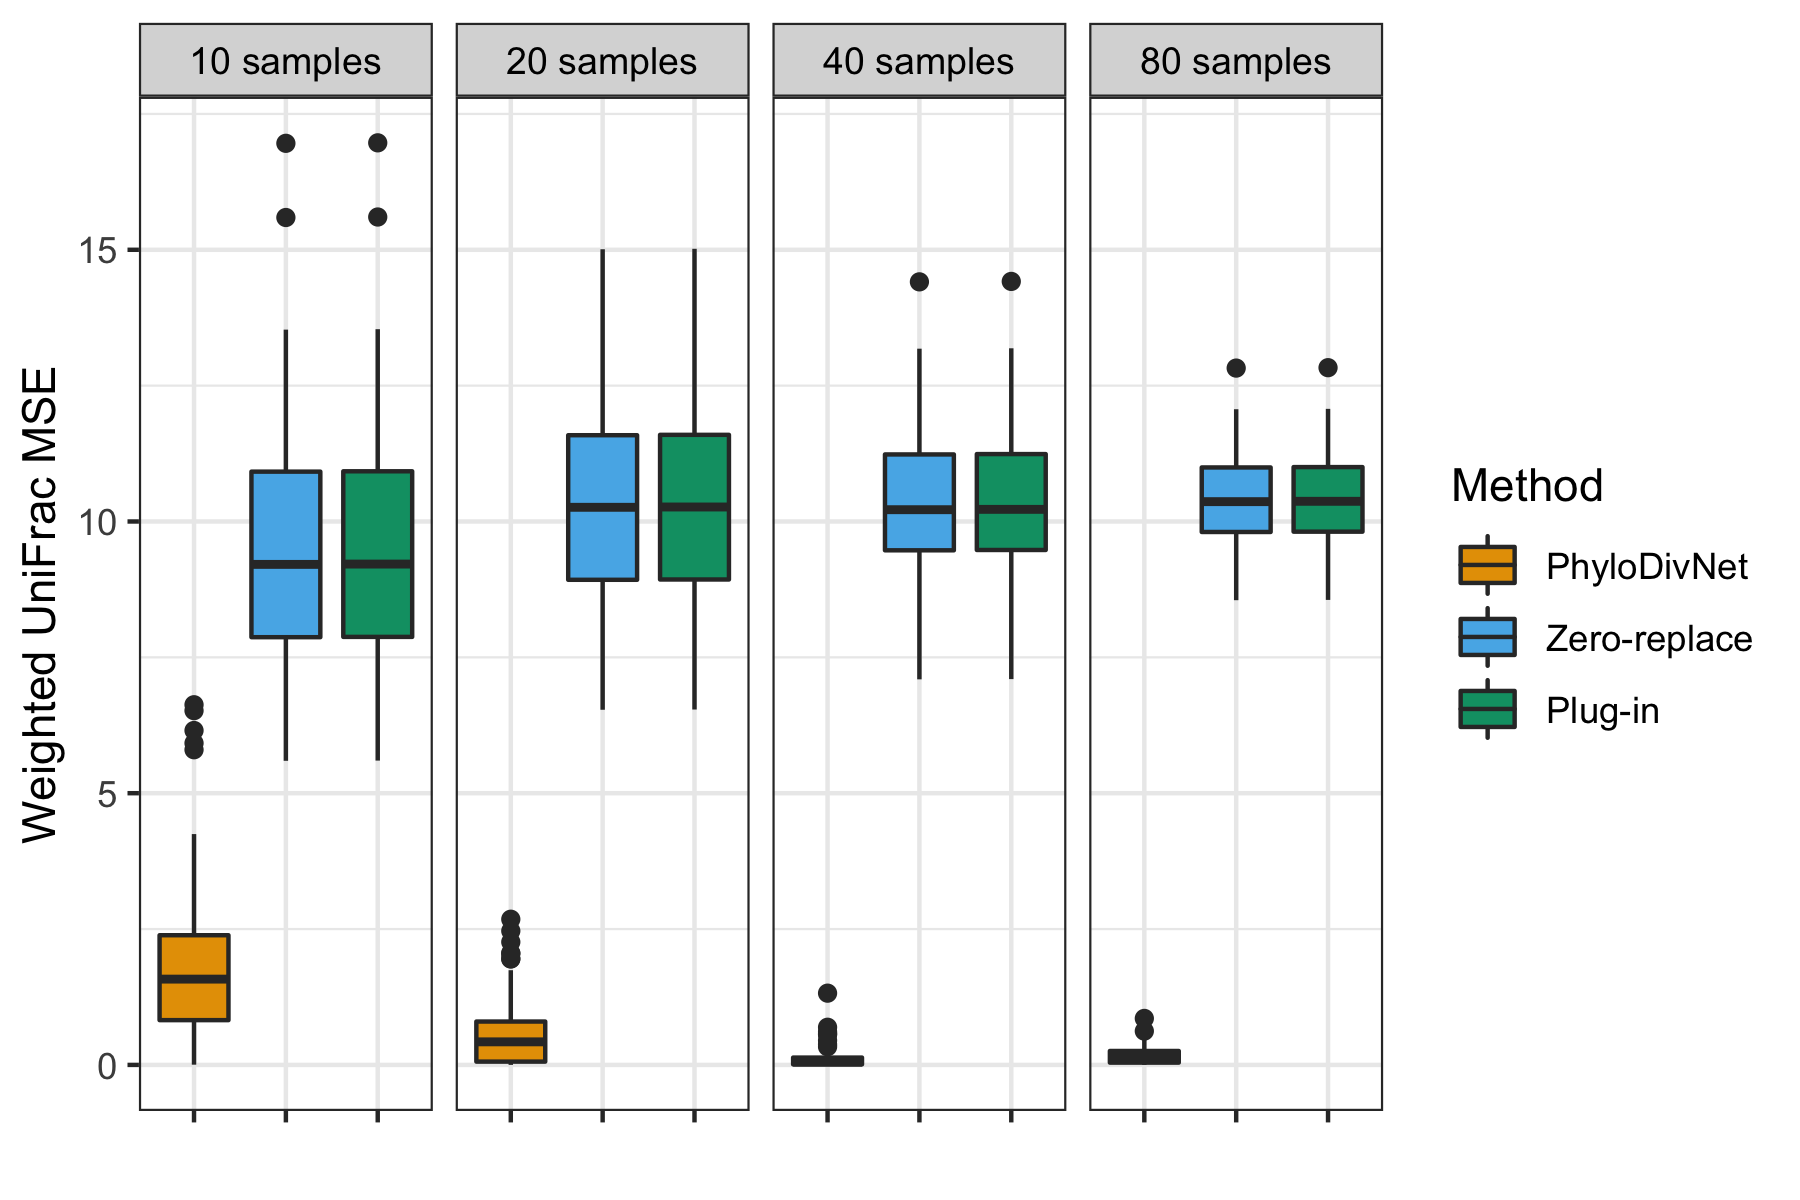
\includegraphics[width=\textwidth]{n_vary.png}
\end{figure}

Figure 1 illustrates the performance of {\myfont PhyloDivNet} against the \textit{zero-replace} and \textit{plug-in} estimators using the MSE. Increasing sample size results in lower estimation error when using {\myfont PhyloDivNet}, but the same pattern does not hold for the \textit{zero-replace} and \textit{plug-in} estimators. This is expected as these estimators do not utilize information from the covariate matrix in their estimation approaches and thereby do not benefit from the increased information afforded with larger sample sizes. Additionally, for all values of $n$ we see that the estimation error of {\myfont PhyloDivNet} is uniformly lower than the estimation error of the \textit{zero-replace} and \textit{plug-in} estimators.  These results are consistent with {\myfont DivNet}'s estimation of non-phylogenetic $\alpha$ and $\beta$ diversity metrics (Willis and Martin [Under Review]). 

\subsubsection{Estimation Error is Small and Stable With Increasing Number of Taxa}
We next investigate the performance of {\myfont PhyloDivNet} against the \textit{zero-replace} and \textit{plug-in} estimators with varying number of taxa. For these simulations we set $n = 30$, $\sigma_{min} = 0.01$, $\sigma_{max} = 5$, $M_{i} = 10^5$ for all $i$, $K$ = 50 simulations, and evaluate four different community sizes $Q = 20, 50, 150, 300$. An input phylogenetic tree for each simulated set of $Q$ was constructed using the {\myfont rtree} function from {\myfont ape} (Paradis 2004) where $Q$ taxa are specified and the edges of the tree are randomly split until $Q$ tips have been reached. The branch lengths of the tree are drawn from a Uniform(0,1).

\begin{figure}[!htb]
 \captionsetup{singlelinecheck = false, format= hang, justification = raggedright, font = sf, labelsep = space}
  \caption{Normalized Weighted UniFrac: Q-vary}
  \centering
  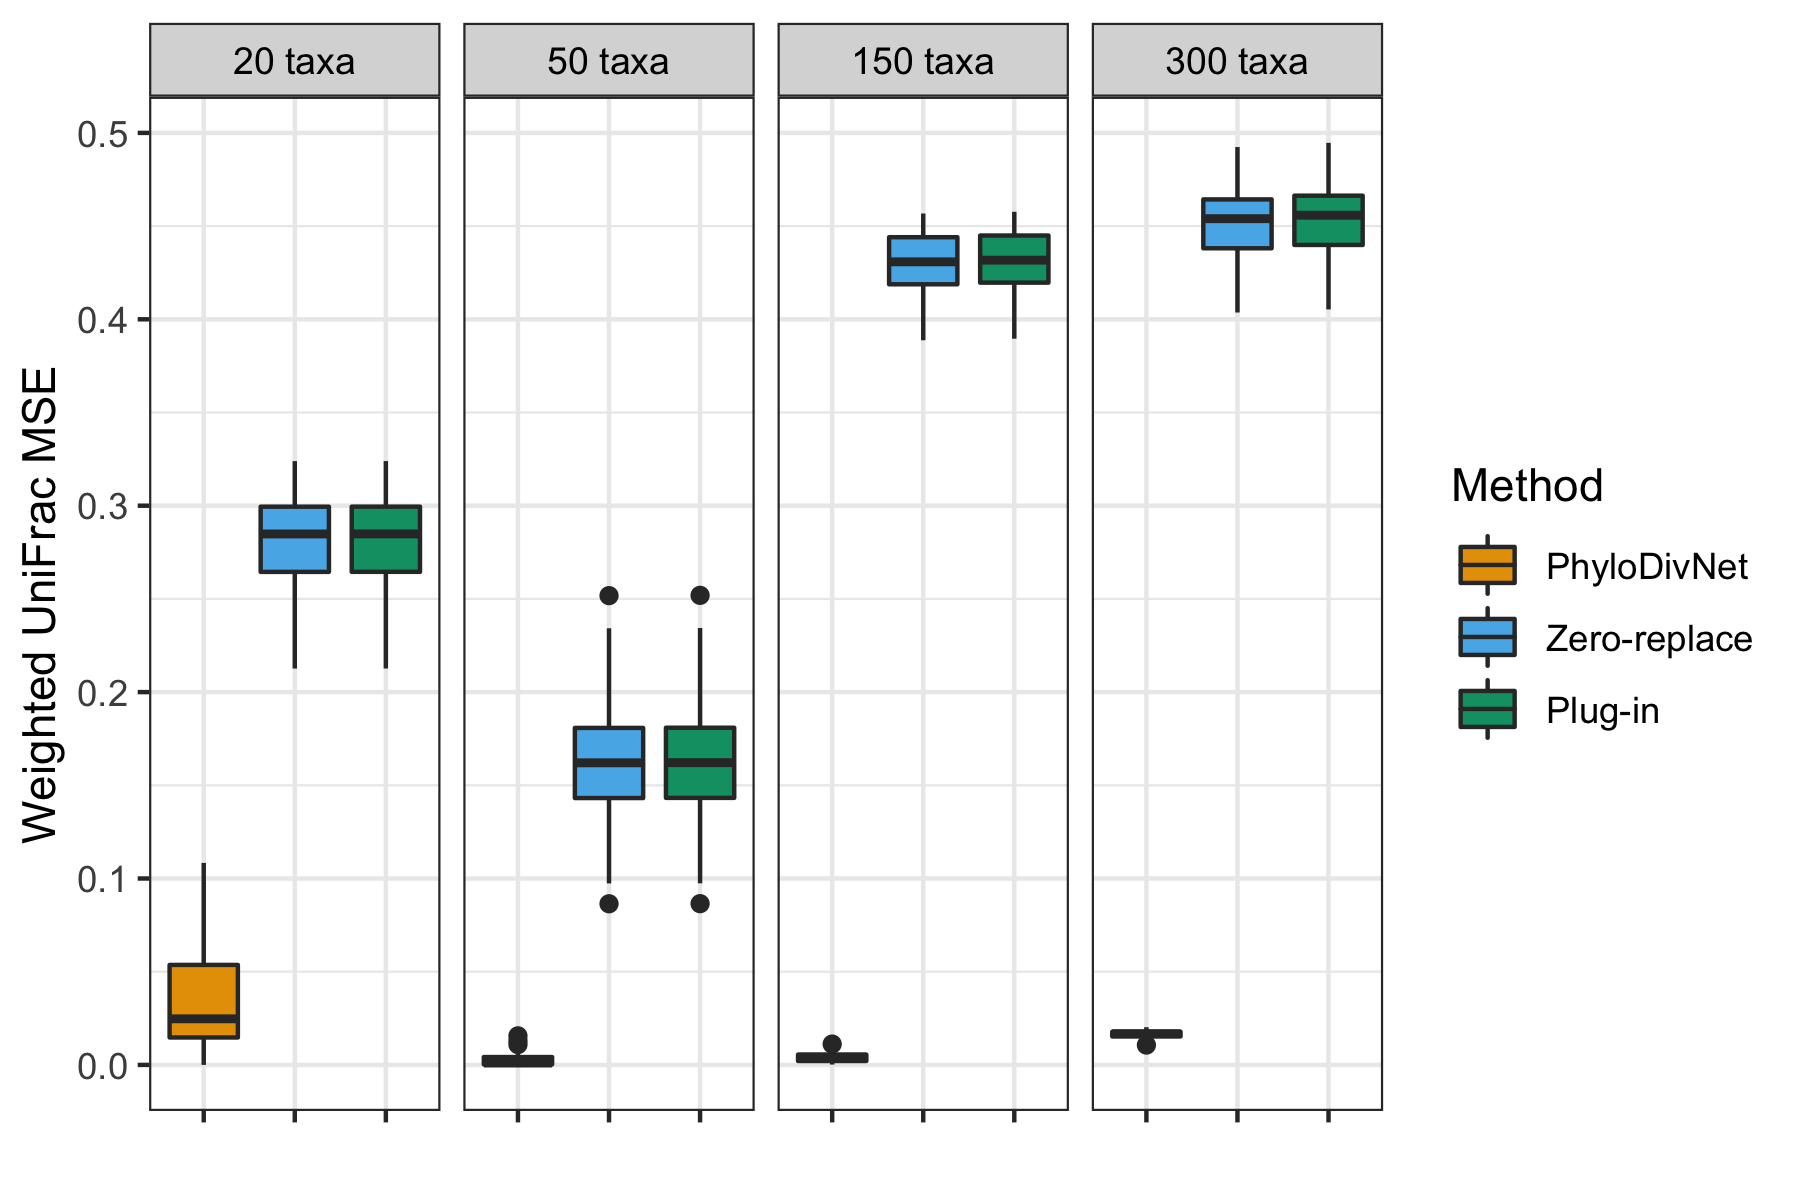
\includegraphics[width=\textwidth]{q_vary.png}
\end{figure}

Figure 2 shows the simulation results. We see that with increasing number of taxa {\myfont PhyloDivNet} maintains smaller estimation error than both the \textit{plug-in} and \textit{zero-replace} estimators. In fact, in all community sizes the 75th quantiles of ${MSE(\widehat{UniFrac}^{(k)})}_{k}$ for {\myfont PhyloDivNet} are uniformly lower than the \textit{zero-replace} and \textit{plug-in} methods. It common in microbiome studies for $q >> n$ and we see that estimation error is typically larger with larger numbers of taxa for the \textit{plug-in} and \textit{zero-replace} methods. Here we demonstrate that {\myfont PhyloDivNet} outperforms the \textit{zero-replace} and \textit{plug-in} methods in estimating the weighted UniFrac in terms of the MSE even in communities with large numbers of taxa. 

\subsubsection{Estimation Error is Small and Stable Across Increasing Strengths of Co-occurrences}
We know that bacteria live in networked communities and that co-occurrence patterns exist between microorganisms that may be due to factors such as shared physiologies, habitat affinities, or functional ecological roles (Barber\'an et al. 2012). As such, a method for estimating diversity that can take into consideration co-occurrences would be appropriate for microbial community analysis. We investigate the estimation performance of {\myfont PhyloDivNet} with differing networks of microbial co-occurrences by examining different $\sigma_{max}$. $\sigma_{max}$ refers to the maximum eigenvalue of a $\Sigma$ matrix where larger eigenvalues correspond to stronger co-occurrences. For our simulations we set $Q = 50$, $n = 30$, $\sigma_{min} = 0.01$, $M_{i} = 10^5$ for all $i$, $K$ = 100 simulations, and evaluate four strengths of co-occurrences $\sigma_{max}$ = 0.1, 5, 10, 15. An input phylogenetic tree is constructed for each simulated set of $\sigma_{max}$ was constructed using the {\myfont rtree} function from {\myfont ape} (Paradis 2004) where $Q$ taxa are specified and the edges of the tree are randomly split until $Q$ tips have been reached. The branch lengths of the tree are drawn from a Uniform(0,1). Figure 3 displays the results of our simulation. 
\begin{figure}[!htb]
 \captionsetup{singlelinecheck = false, format= hang, justification = raggedright, font = sf, labelsep = space}
  \caption{Normalized Weighted UniFrac: Sigma-vary}
  \centering
  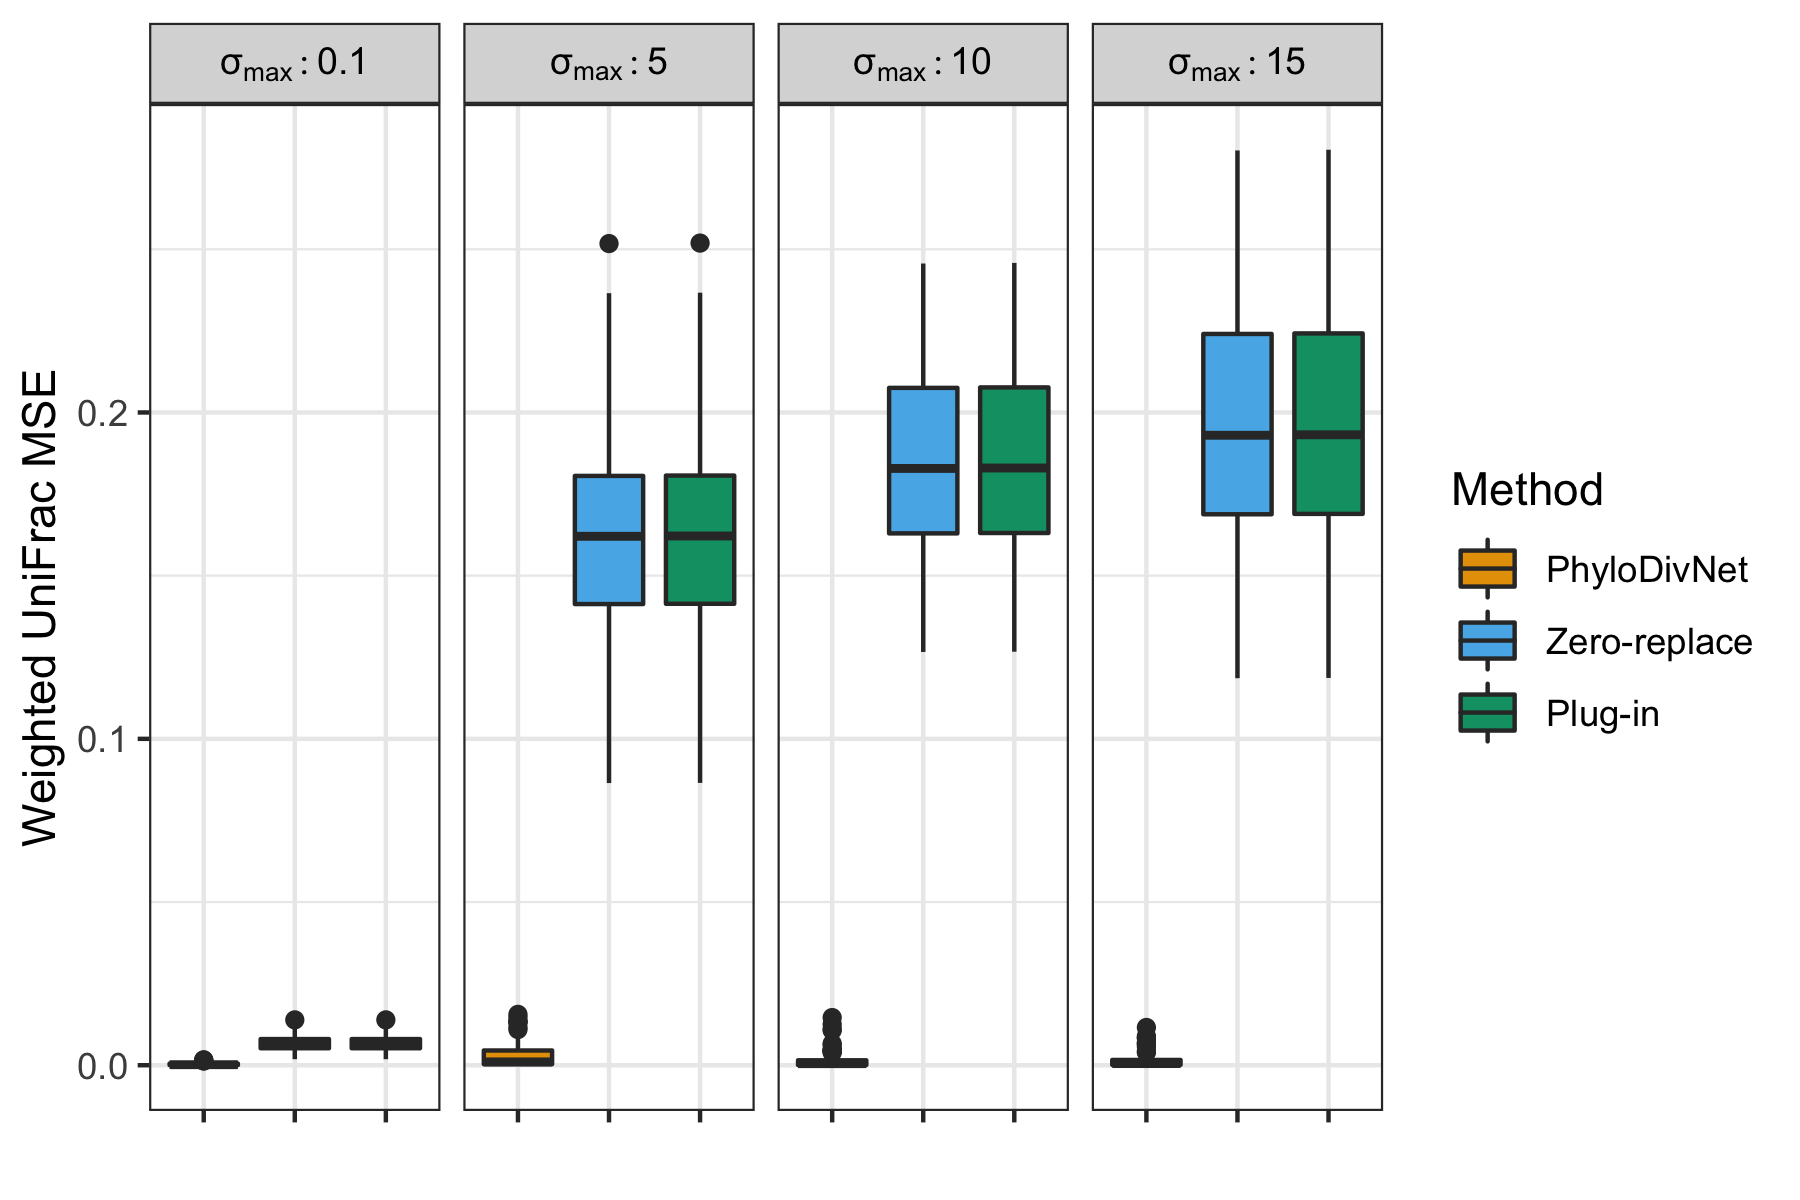
\includegraphics[width=\textwidth]{s_vary.png}
\end{figure}

We observe that with stronger co-occurrences the estimation error increases for the \textit{zero-replace} and \textit{plug-in} estimators whereas {\myfont PhyloDivNet}'s estimation error remains consistently smaller. We thus conclude that {\myfont PhyloDivNet} is well suited for estimating weighted UniFrac in the presence of strong and weak microbial co-occurrence networks. 

\subsubsection{Unbalanced versus Balanced Trees}
\begin{figure}[!htb]
    \centering
    \captionsetup{singlelinecheck = false, format= hang, justification = raggedright, font = sf, labelsep = space}
    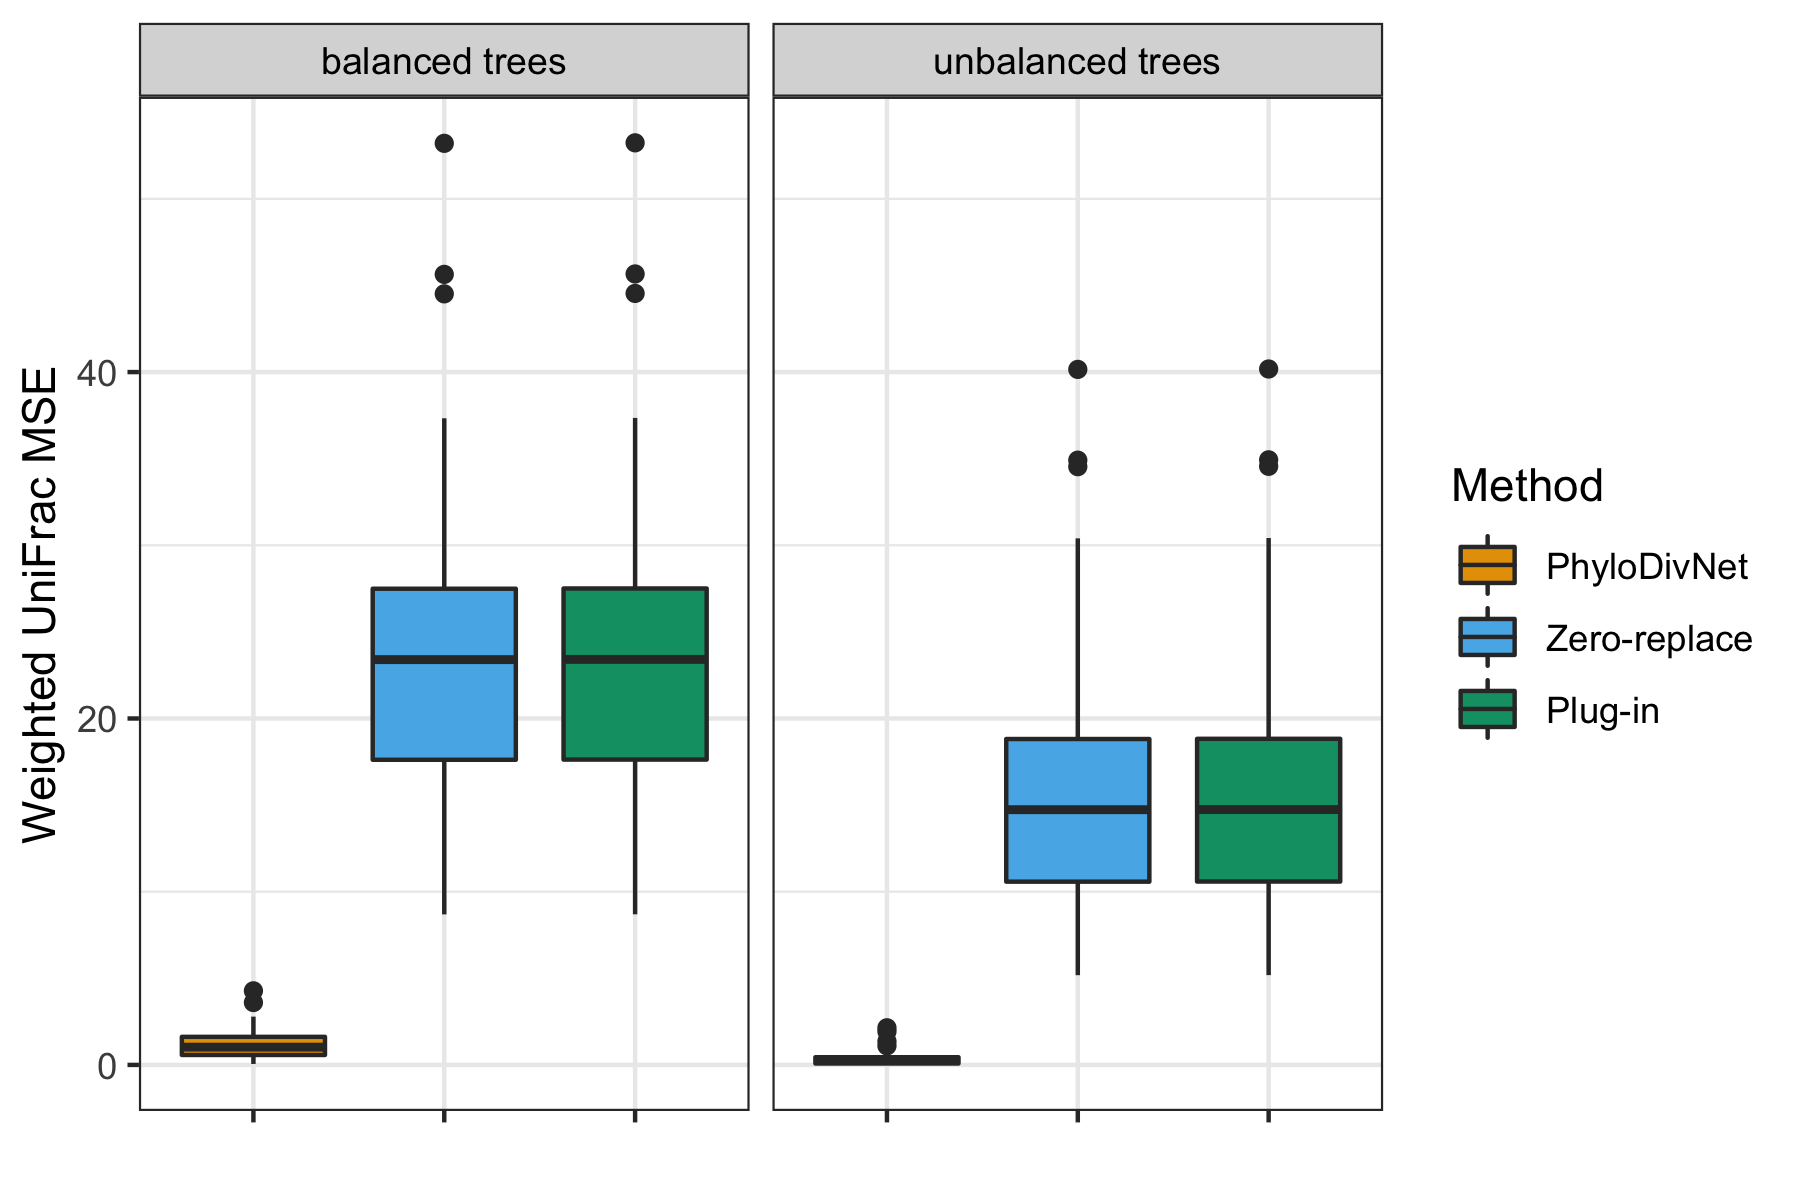
\includegraphics[width=\textwidth]{tree_vary.png}
    \caption{Weighted UniFrac: tree vary}
    \label{fig:my_label}
\end{figure}

The MSE is so big for the plug-in and zero-replace methods! 


\subsection{Variance Estimation Simulation}
Compare nonparametric vs. parametric bootstrap. Use the naive approach to estimating the covariance. Comparison of the two bootstrap methods. 
The parameter $\Sigma$ drives the variance in the log-ratio model 
\begin{figure}[!htb]
 \captionsetup{singlelinecheck = false, format= hang, justification = raggedright, font = sf, labelsep = space}
  \caption{Variance Estimation Plot}
  \centering
  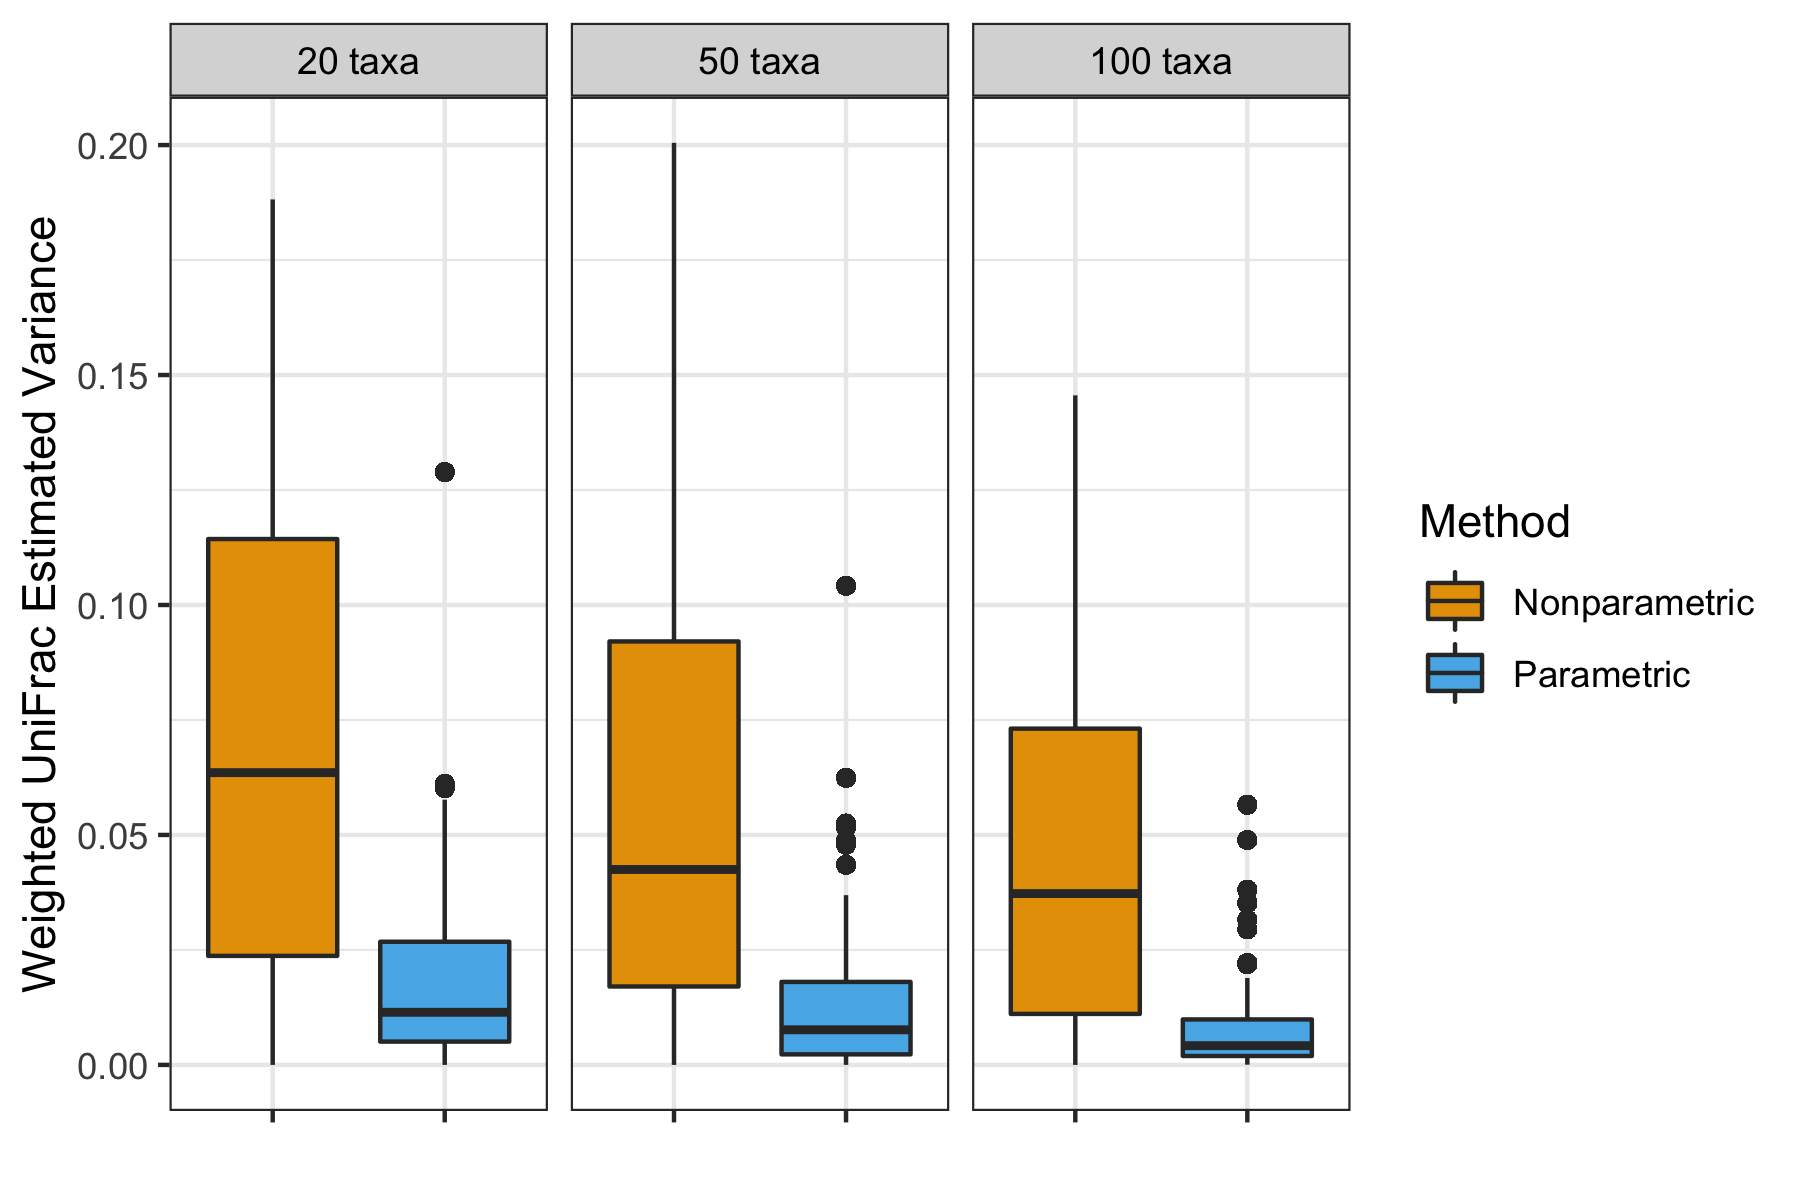
\includegraphics[width=\textwidth]{variance_estimate.png}
\end{figure}

\begin{figure}[!htb]
 \captionsetup{singlelinecheck = false, format= hang, justification = raggedright, font = sf, labelsep = space}
  \caption{Variance Estimation Difference Plot}
  \centering
  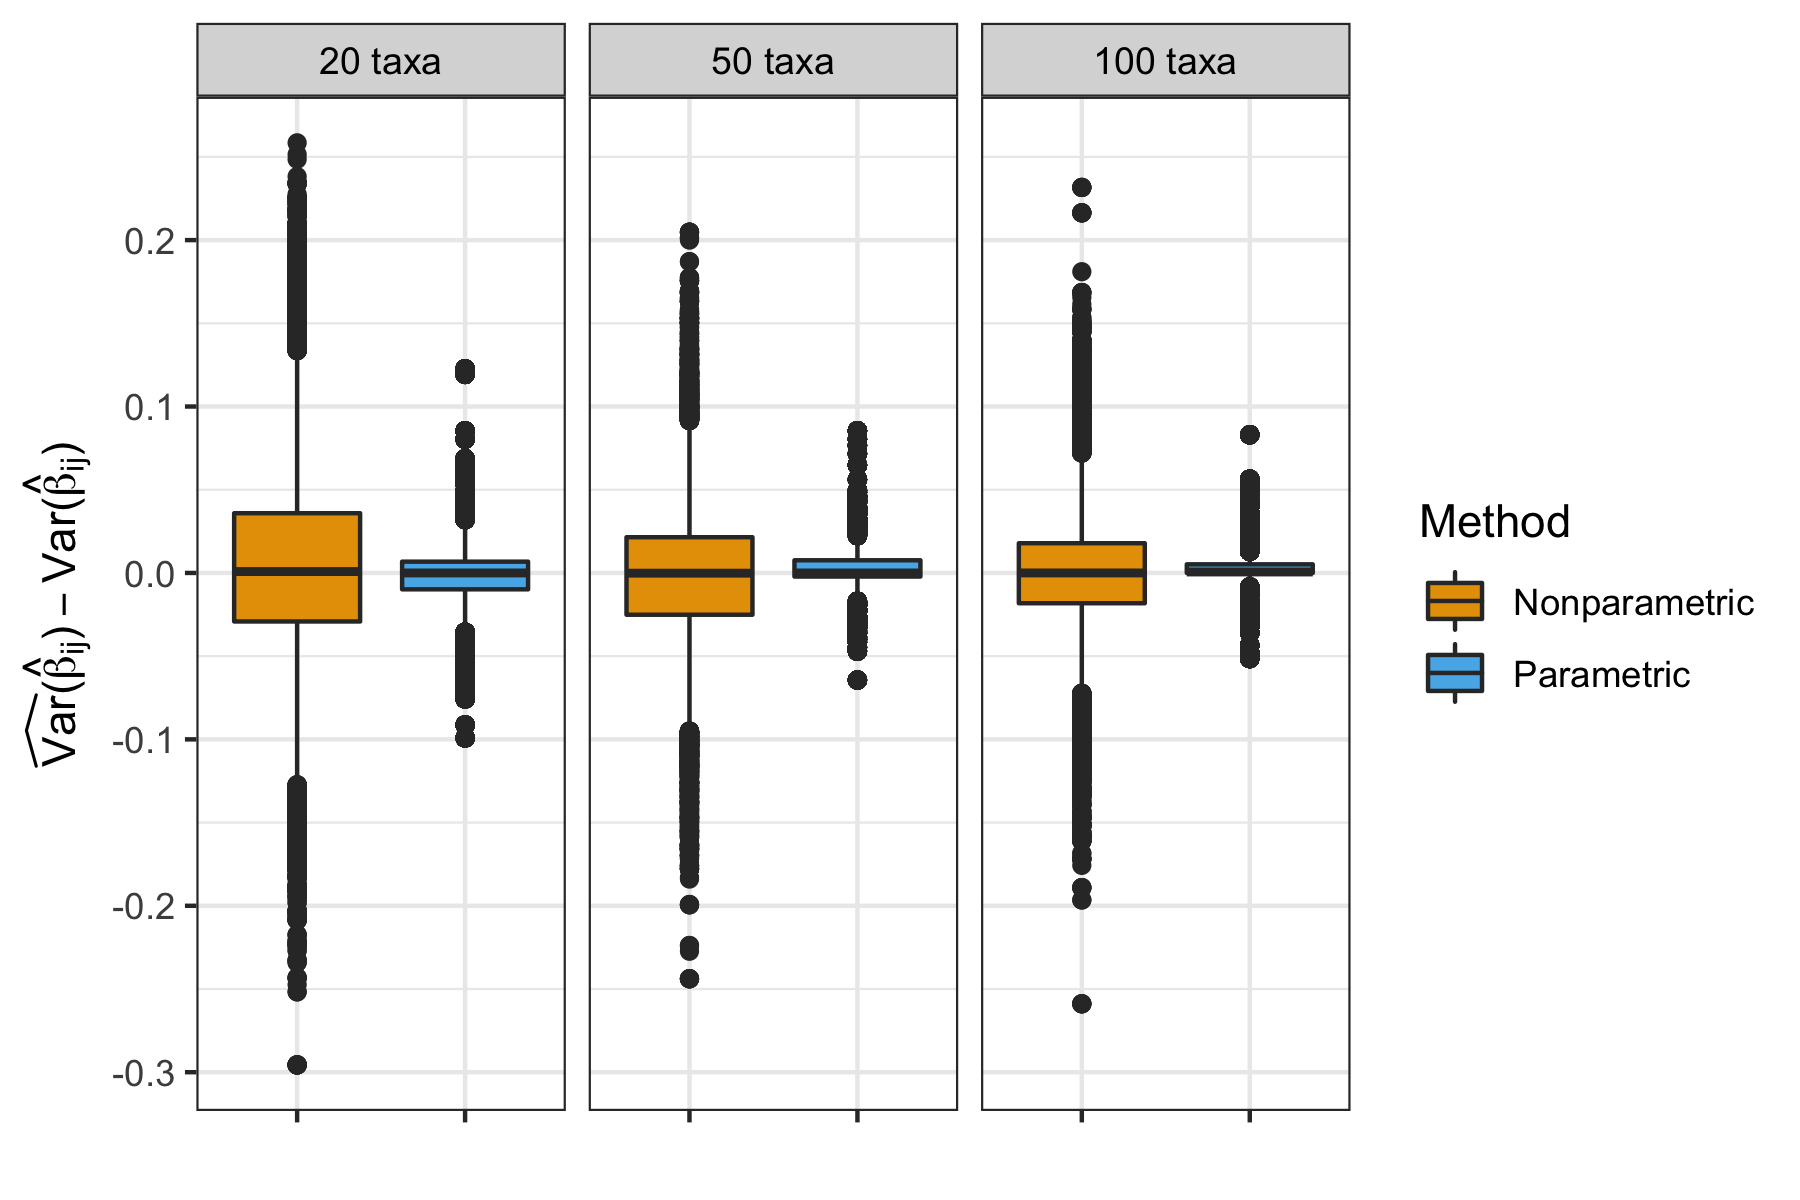
\includegraphics[width=\textwidth]{variance_diff.png}
\end{figure}

\subsection{Data Analysis}
- Talk about the pre-processing 
- How many bootstrapped estimates are we generating? 100 
- 
\begin{figure}[!htb]
 \captionsetup{singlelinecheck = false, format= hang, justification = raggedright, font = sf, labelsep = space}
  \caption{Data Analysis Results}
  \centering
  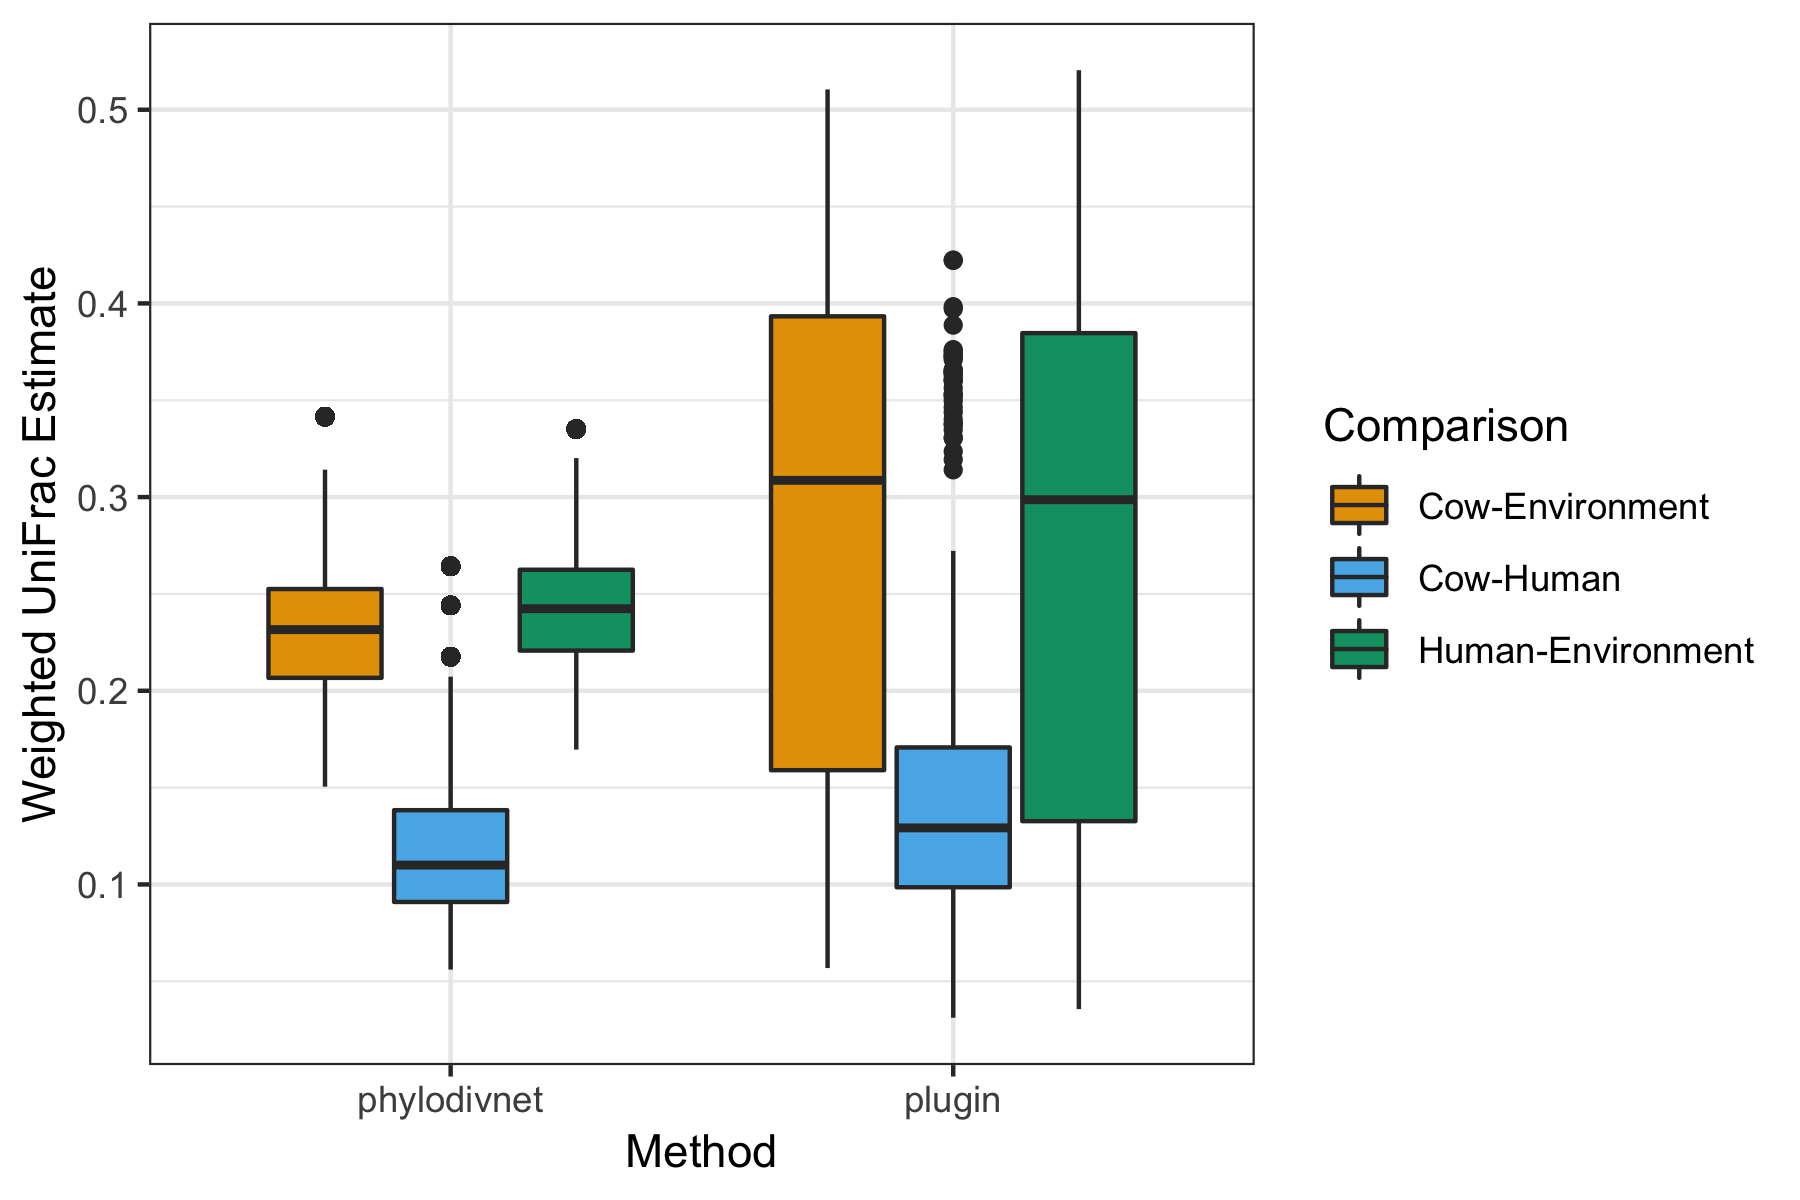
\includegraphics[width=\textwidth]{HDWanalysis_plots_B100.png}
\end{figure}

\subsection{Hypothesis Testing}
what is currently being done is that UniFrac is calculated and then Monte Carlo Simulations are done to see whether or not the fraction of the tree unique to one environment is greater than would be expected by chance. 

\subsection{Discussion}
{\myfont github.com/statdivlab/PhyloDivNet} 

\section{Follow-up/To Do}

\begin{itemize}
    \item Results of Simulation 
    \item Introduction 
    \item Discussion
\end{itemize}

\section{Notes}
\begin{itemize}
    \item Validation of Estimates 
    \subitem Differing q's 
    \subitem Differing sample sizes 
    \subitem Differing types of trees 
    \subitem Different correlation structures 
    
    Estimation error is stable across large communities and stable across different networked communities. Estimation error decreases with increased sample size. 
What type of trees do I want to test? 
\end{itemize}

\bibliographystyle{plain}
\bibliography{references}
Mart\'in-Fern\'andez 2003 https://link.springer.com/content/pdf/10.1023%2FA%3A1023866030544.pdf

Vu 2007 
https://statistics.berkeley.edu/sites/default/files/tech-reports/727.pdf

Paradis 2004 
https://cran.r-project.org/web/packages/ape/index.html

Barber\'an https://www.ncbi.nlm.nih.gov/pmc/articles/PMC2728295/

Simulation conditions are p = 3;  n = 80, 40, 20, 10; q = 50; $\sigma_{min}$ = 0.01, $\sigma_{max}$ = 5; n = 100 simulations 

Simulation conditions are p = 3; q = 20, 50, 150, 300; n = 30; $\sigma_{min}$ = 0.01, $\sigma_{max}$ = 5; nsim = 50 

Simulation conditions are p = 3; q = 50; n = 30; $\sigma_{min}$ = 0.01; $\sigma_{max}$ = 0.1, 5, 10, 15; nsim = 100 


\end{document}
